\chapter{Introduction}\label{sec:Introduction}
\pagenumbering{arabic}
\setcounter{page}{1}
As the technology evolves it unlocks more and more possibilities. Just a few years back there were no smartwatches or phones but at this time they are important part of our lives. As they evolve there is the need for them to have more functions and features. One of these features is to be able to locate its position on the map. This information is very useful since it can prevent people from getting lost, figuring out path to drive, used by military and in countless more cases.

Finding such position is possible using Global Navigation Satellite System (GNSS). Multiple implementations of this system exist, such as GPS, GLONASS or Galileo. All of these systems provide location using sufficient number (at least four) of satellites \cite{GNSS, GNSSGPS}. GNSS solution requires clear line of sight between satellites and the receiving device because signal is not able to pass through buildings. This makes it the main reason why it cannot be used for indoor localization.

\begin{figure}[h!]
	\begin{centering}
		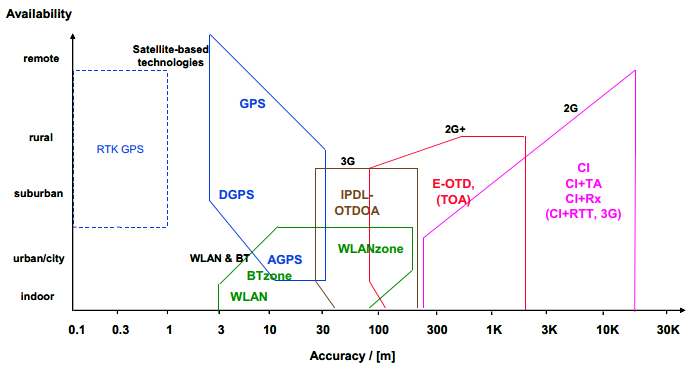
\includegraphics[width=0.7\textwidth]{img/1_comparison_of_positionin_technologies}
		\par\end{centering}
	\caption{Comparison of Positioning Technologies (source: \cite{PedestrianDeadReckoning})\label{fig:1_comparison_of_positionin_technologies}}
	\label{fig01c01}
\end{figure}

There are multiple approaches to find out location inside the building. They can be divided into three main types. First, using wireless signal ranging approach with multiple kinds of data such as Time of Arrival (ToA). Second, using special equipment like active bats (Ultrasonic). Final, based on Signal Strength Fingerprint Maps (SSFM), in which first part is to collect signal strengths from the environment and construct fingerprint maps. These maps are then used to match with current signal to obtain device location \cite{LocalizationApproaches}.

In addition to these types of localization there are also multiple algorithms used in indoor environments. Some of them are location fingerprinting, triangulation, proximity and dead reckoning \cite{AaPLocalisation}. Few of these algorithms will be described in \hyperref[sec:LocalizationTechniques]{Chapter 2}.

This thesis is focused on method using radio signal strength (RSS) fingerprinting by collecting data from Bluetooth, wireless and cellular devices.

\section{Goals of this thesis}\label{sec:GoalsOfThisThesis}
Main goal of this thesis is to explore possibilities of fingerprint acquisition using smartwatch technology. The first question that needs to be answered is if this can be done. Is smartwatch capable of RSS data collection? And the answer to this question is yes, since smartwatches have the similar specifications as low-end smartphones, containing Bluetooth and WiFi chips, which means it can be done. 

One of the goals for this thesis is to create an application for Android phone and wear device which handles RSS fingerprint collection. Problem with smartwatches is their diversity in operational systems because a lot of watch creators have their own custom systems which can complicate things. Luckily there is a version of Android operating system called WearOS (used to be Wear 2.0) and it is basically a port of Android system to wearable devices. 

Final goal is to test created application and figure out if data from wear device increase precision of indoor localization or not.

\section{Reason for selection of this topic}\label{sec:ReasonForSelectionOfThisTopic}
The reason behind selection of this topic is rather simple. I was introduced to Android during my studies at the University Hradec Králové but it was just basic knowledge. That is why I later decided to go for a study abroad to deepen my knowledge. Part of that study was to work for a selected company where we developed rather complex Android application. Its core part was using multiple APIs, user authentication and data encryption but it was still focused only on a singe device, that being the phone. So next thing I wanted to try was working with multiple kinds of devices and since WearOS is rather new I wanted to test it out. So the main reason is to get more experienced with Android and as a developer.